\chapter{Setup and Implementation}
\label{chap:3}
%
\gls{ROS} simulation environment was used for testing approaches. \gls{ROS} is a framework where testing cases can be easily developed and tested. In a current simulator, there are few small environments imitated consisting of a static map (T and X intersection) and the car itself. \\
In order to visualize simulation \gls{RViz} which is s a 3D visualizer for showing data and state information from \gls{ROS} was used. A snapshot of the simulation environment is in Figure~\ref{fig:ROS1}. The code was written in Python and C++ programming languages.

\begin{figure}[h]
	\centering  	
	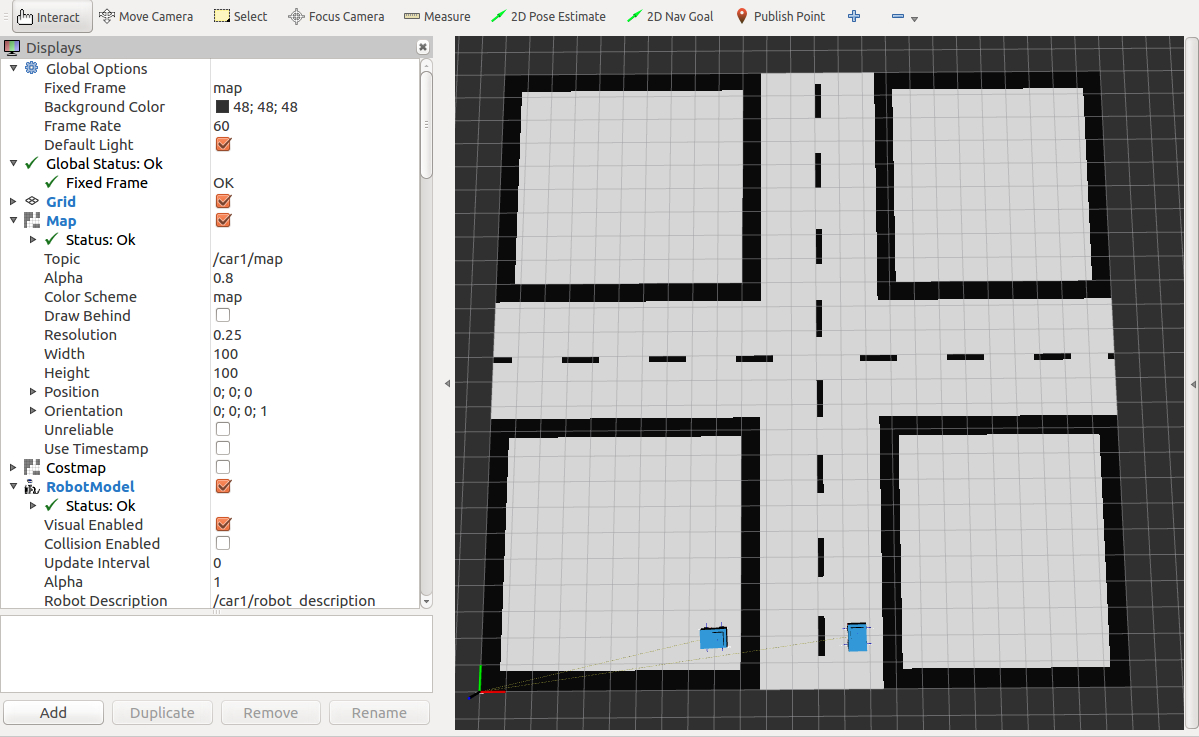
\includegraphics[width=10cm]{img/Ros.jpg}
	\caption{The \gls{RViz} environment that runs the simulation, having X-Intersection in mind}
	\label{fig:ROS1}    
\end{figure}

For this project, several testing cases were developed. Methods tested offline (with having all trajectory for testing) and online (having only current and last position). Data from every run is stored in order to analyze it and see how each method effect performance of the system.
Parameters and results for each trajectory are independent and tested several times in a specific environment to be able to draw conclusions from the results we received during the testing.

\section{Data Collection}

To be able to test our approach database of various trajectories need to be used. To make our own database for possible trajectories and not to use already existing data was taken at the beginning stage of this project. Due to that data collection was one of the first steps after all simulation environment was set. \\

To be able to control car in \gls{ROS} environment and record data joy package was used. Joy package is a \gls{ROS} driver for a "generic Linux joystick".The package consists of joy\_node, a node which allows communication between a generic joystick and \gls{ROS}. Joy message, which contains information about the current state of each button on joystick is published by node \cite{ROSjoy}, having this information command start to move, turn to any direction, stop is sent to the object we want to control in \gls{ROS} environment. When an object, the car in our car is able to move in \gls{ROS} using a joystick we recorded and stored a car's position every few milliseconds. \\

For each map type, slightly different types of trajectories were recorded. For X-intersection a various number of trajectories for movement to the right, straight and left were recorded, while for T-intersection only movement t the right and left was recorded.

\section{Brief Algorithm Explanation}

In this section a brief overview of the main code algorithm for getting test results will be explained.

\subsection{Map Recognition}

In this project, two \textcolor{red}{(so far)} maps, imitating X and T intersection, were used. Map recognition is necessary because the further calculation is a bit different on T and X intersection maps. \\
The map is recognized using .... \textcolor{red}{Not exactly sure if I will leave current map recognition algorithm, where I am using simple contour recognition or will go to a more complicated one. That's why here I left this section empty.}

\subsection{Trajectories' Unification}

The problem with our current database is that there are a lot of trajectories which have a different number of time steps. This happened because of different trajectory length (e.g. to go straight takes less time and it is a less distance than going to left or right), the velocity of the car may differ in each or even in the same trajectory (velocity depends on control of the joystick), etc. Having different time steps in trajectories makes some problems in further calculations, comparison of results, the calculation over thousands of steps also has a longer computation time, etc. Because of that trajectories, unification is a necessary step. \\

Unification made using interpolation when all trajectories transformed to have an equal number of time steps, in spite of the original number of time steps. This is achieved by interpolation, in mathematics interpolation is a method of building new data points inside the range of a discrete set of known/given data points. \\

The pseudo code below (Figure~\ref{fig:pseudoInter}) shows the way of interpolation in this project.

\begin{figure}[h]
	\centering  	
	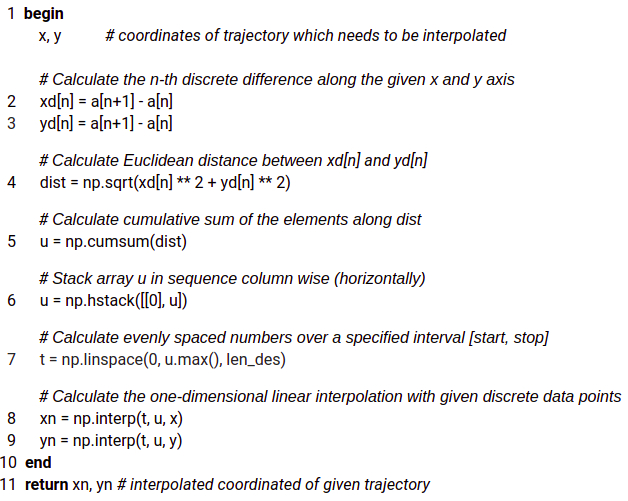
\includegraphics[width=13cm]{img/interpolation.jpg}
	\caption{Pseudo code for interpolation \textcolor{red}{(need to rewrite it to make it pseudo)}}
	\label{fig:pseudoInter}    
\end{figure}

Figure~\ref{fig:InterExam} shows 3 original trajectories and interpolated version of the same trajectories. Original trajectory, which goes to the right has $7,581$ time steps, while straight trajectory has $13,666$ and the left trajectory has $10,929$ time steps after interpolation all trajectories contain 10 steps (number of time steps can be changed according to preference or test case).

\begin{figure}[h]
	\centering  	
	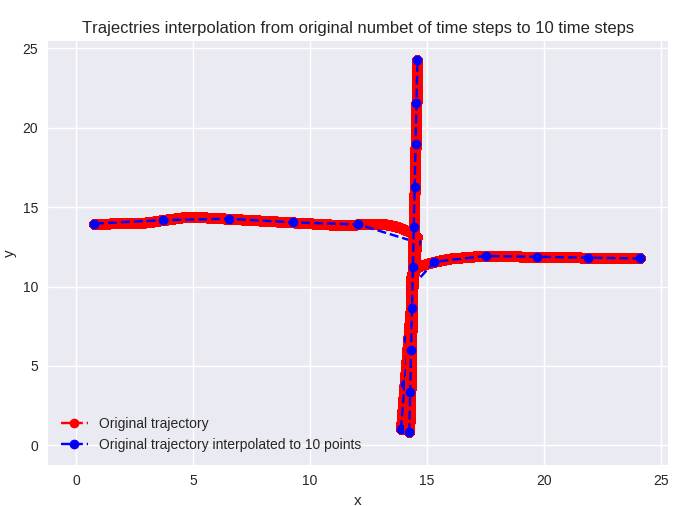
\includegraphics[width=10cm]{img/interpolation_example.jpg}
	\caption{Original and Interpolated Trajectories}
	\label{fig:InterExam}    
\end{figure}

As can be seen, interpolation does not ruin trajectories and can be used in further calculations.

\section{Modeling Belief for Prediction Making}

A Bayesian version of a Gaussian mixture model is used for calculating the belief for each trajectory class and this section gives definitions for beliefs representing for a car over trajectory classes (going right, going straight, going left). Since we can only observe the current position of the car, which means that trajectory class is partially observable, due to that our belief is represented as a probability distribution over all trajectory classes. \\

For maintaining correct belief, belief update must be done every time step. Updating belief constantly is important because of sudden position change can show drivers' intentions and what his next steps could be. To be able to predict possible future movement current position information need to consider every time when belief update is calculated. The belief update is calculated using Bayes rule formula~\ref{eqn:formula1} below: 

\begin{equation}
\begin{split}
b_{t+1}(k) = & \displaystyle Pr(k|o_{t}, b) \\ 
& = \displaystyle \frac{Pr(o_{t}|k, b) Pr(k|b)}{Pr(o_{t}|b)} \\
& = \displaystyle \frac{Pr(o_{t}|k, b) Pr(k|b)}{ \sum_{k} Pr(o_{t}|b) Pr(k|b)} \\
& = \displaystyle \frac{Pr(o_{t}|k, b) b_{t}(k)}{ \sum_{k} Pr(o_{t}|b) Pr(k|b)}
\end{split}
\label{eqn:formula1}
\end{equation}

With given formula belief for future step $b_{t+1}(k)$ for a predefined class is calculated. $Pr(o_{t} | k, b)$ is the car position observation model, which returns the probability (or likelihood) of going to any direction from the current position, observed with $o_{t}$. This likelihood can be calculated using multivariable Gaussian probability distribution function f(x,$\mu$,$\Sigma$). This probability distribution function looks the following:

\begin{equation}
\begin{split}
f(x,\mu,\Sigma) = \displaystyle \frac{1}{\sqrt{(2 \pi)^n det(\Sigma)}} exp(-\frac{1}{2}(x-\mu)^T\Sigma^{-1}(x-\mu)), 
\end{split}
\label{eqn:formula2}
\end{equation}

where dimensionality n = 2 and x is a currently observed position of the car $x = (o_t^x, o_t^y)^T$, $\mu$ is a mean from all predefined trajectories in data base for the same class $\mu_k  = (\mu_{t,k}^x, \mu_{t,k}^y)^T$ and $\Sigma$ is a covariance matrix of all predefined trajectories in data base for the same class $\Sigma_k  = (\Sigma_{t,k}^x, \Sigma_{t,k}^y)^T$.Mean for x and for y coordinates can be found using formula~\ref{eqn:meanX} and formula~\ref{eqn:meanY} respectively:

\begin{equation}
\begin{split}
f(\mu_x) = \displaystyle \frac{\sum_{i=1}^{n} x_i}{n}
\end{split}
\label{eqn:meanX}
\end{equation}

\begin{equation}
\begin{split}
f(\mu_y) = \displaystyle \frac{\sum_{i=1}^{n} y_i}{n}
\end{split}
\label{eqn:meanY}
\end{equation}

Covariance value can be calculated using formula~\ref{eqn:COV}

\begin{equation}
\begin{split}
f(\Sigma_{x.y}) = \displaystyle \frac{\sum_{i=1}^{n} (x_i - \mu_x)(y_i - \mu_y)}{n-1}
\end{split}
\label{eqn:COV}
\end{equation}

The denominator of formula~\ref{eqn:formula1} is the so-called normalization factor, which sums all likelihoods of the car over all movement classes at the current time step. The final result of formula will return updated belief that car is moving towards any of classes. \\

Figure~\ref{fig:PseudoBelief} shows pseudo-code how belief updates are made over time, as an input having current belief $b_t$ at time step t, current car position $x_t, y_t$ from the last made observation, as well we have before calculated mean and covariance values at that time, $\mu_{t,k}^x, \mu_{t,k}^y$ and $\Sigma_{t,k}^x, \Sigma_{t,k}^y$ respectively.

\begin{figure}[h]
	\centering  	
	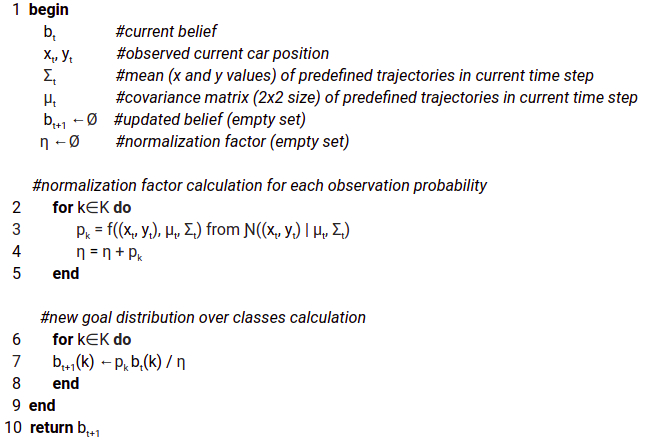
\includegraphics[width=13cm]{img/pseudo_belief update.jpg}
	\caption{Pseudo Code for Updating belief}
	\label{fig:PseudoBelief}    
\end{figure}

\section{Trajectory Scaling}

Computation time for prediction is one of the main things which needs to be fast. Even though more belief updates give more precise results, more computations take more time. In this project, we took various numbers of time steps and compared results to get them as precise as possible and have fewer time steps (e.g. we aimed to keep precision of trajectory of 100-time steps but have only 10-time steps trajectory). \\

There were a lot of various trajectories with various numbers of points, but with an original approach result still was that with more time steps prediction results were more precise. Later on, Toy Problem approach came into the sight. \cite{ToyPr} defines it as "In scientific disciplines, a toy problem is a problem that is not of immediate scientific interest, yet is used as an expository device to illustrate a trait that may be shared by other, more complicated, instances of the problem, or as a way to explain a particular, more general, problem-solving technique". \\

After unsuccessfully trying different methods, the idea of raising a likelihood (formula~\ref{eqn:formula2}) of the trajectory with a bigger number of time steps at every time step by $\frac{1}{\frac{bigger number of time steps in trajectory}{smaller number of time steps in trajectory}}$ and then compare results of matching points in each trajectories. \\

To simplify all this, let's have an example: let's imagine we have the trajectory interpolated to 100-time steps and we want to see how results differ when we do belief updates all 100 times with doing belief at every 10th step (10th, 20th, ..., 90th, 100th). Without doing any changes in the original code, these results are not matching, in fact, they differ quite a lot. But if we raise likelihood (formula~\ref{eqn:formula2}) of the trajectory where belief is updating 100 times by $\frac{1}{\frac{100}{10}} = \frac{1}{10}$ at every time step and then do belief updates as normal and compare them with belief updates which are calculated every 10th step with making no changes in the original code. After comparison of these results, it was easy to see that results are matching or are close enough to each other. The pseudo code of the given example is in Figure~\ref{fig:PseudoScalling}.

\begin{figure}[h]
	\centering  	
	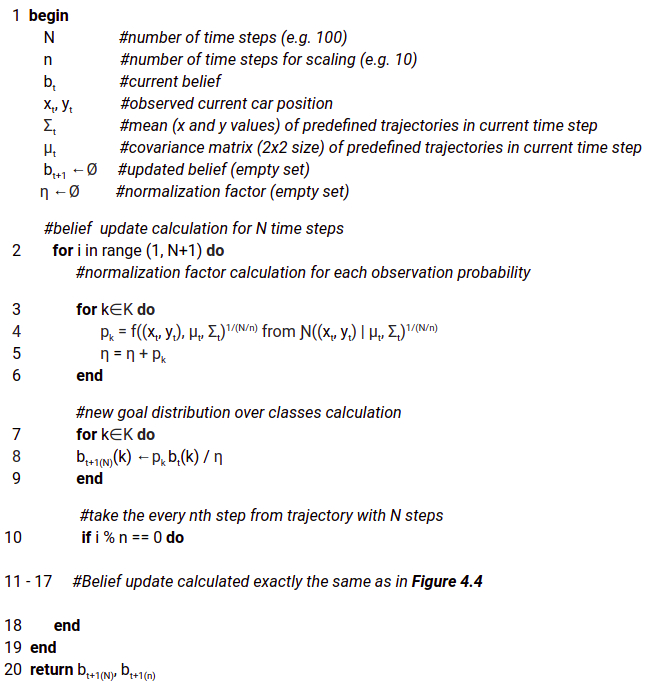
\includegraphics[width=13cm]{img/Pseudo4Scalling.jpg}
	\caption{Pseudo Code for Scaling Trajectory for Belief Update}
	\label{fig:PseudoScalling}    
\end{figure}

Having this in mind we can make our prediction making the process faster and more precise. 

\section{Online Method for Prediction Making}

The online method uses the same, previously described techniques and principles for calculation. The predefined database with trajectories exists, calculations and all preparation for a future working with them are made as well. The one difference between online and offline methods is that all testing and its results visualizations are happening in \gls{ROS} and \gls{RViz}. And the main difference from an offline method, the online method does not have a whole testing trajectory at the beginning, during testing only past and current steps are known. \textcolor{red}{which makes all interpolation kinda complicated, and I need to discuss that with you on a meeting, maybe I am just don't know something and I am raising a problem when it doesn't exist}. Results of prediction are also highlighted in real time in \gls{RViz} environment.
